\documentclass[12pt]{article}

\usepackage[in]{fullpage}
\usepackage{fancyhdr}

%\usepackage{amsmath}
%\usepackage{amssymb}
%\usepackage{mathtools}
\usepackage{graphicx}

\usepackage[polish]{babel}
\usepackage[T1]{fontenc}
\usepackage[utf8]{inputenc}

\renewcommand{\thesection}{\arabic{section}.}
%\renewcommand*{\arraystretch}{1.25}

\begin{document}

\begin{titlepage}

  \fancyhead{}
  \fancyfoot{}

  \fancypagestyle{empty}{
      \fancyhead[R]{\large{26.10.2016}}
  }

  \vspace*{\stretch{1.0}}
  \begin{center}
    \huge{GRAFIKA KOMPUTEROWA 1}\\
    \huge{PROJEKT LABORATORYJNY 1}\\
  \vspace*{\stretch{0.2}}
    \Large{SPECYFIKACJA}\\
  \vspace*{\stretch{0.2}}
    \Large{EDYTOR WIELOKĄTÓW}\\
  \vspace*{\stretch{0.2}}
    \large\textbf{TYMON FELSKI, C1}\\
  \end{center}
    \vspace*{\stretch{1.0}}   

\end{titlepage}

\section{Instrukcja obsługi programu}
\textbf{Dodawanie wielokąta}\\Wielokąty można dodawać klikając \textbf{LPM}. Na ekranie będą pojawiać się kolejne wierzchołki. Rysowanie zakończy się, jeżeli łamana zostanie zamknięta (postawimy ostatni wierzchołek dostatecznie blisko początkowego). Rysowanie można anulować wciskając \textbf{Escape}.\\[\baselineskip]
\textbf{Przesuwanie wielokąta}\\Wielokąt można przesunąć wciskając \textbf{Shift + LPM} lub \textbf{ŚPM}, gdy kursor znajduje się w środku tego wielokąta. Jeżeli kilka wielokątów się pokrywa, o wyborze decydować będzie kolejność ich rysowania.\\[\baselineskip]
\textbf{Przesuwanie wierzchołka}\\Wierzchołek w narysowanym wielokącie można przesunąć przytrzymując na nim \textbf{LPM}.\\[\baselineskip]
\textbf{Usuwanie wierzchołka}\\Wierzchołek w narysowanym wielokącie można usunąć wciskając na nim \textbf{PPM} i wybierając opcję \textbf{Delete} w menu kontekstowym. Wierzchołki można usuwać, jeżeli ich liczba w wielokącie jest większa od 3, w przeciwnym wypadku zostanie wyświetlony komunikat o błędzie.\\[\baselineskip]
\textbf{Dzielenie krawędzi}\\Krawędź w narysowanym wielokącie można podzielić na dwie, dodając w środku wierzchołek. W tym celu należy wcisnąć na niej \textbf{PPM} i wybrać opcję \textbf{Split} w menu kontekstowym. Ograniczenie podzielonej krawędzi zostanie wówczas usunięte (jeżeli było nadane).\\[\baselineskip]
\textbf{Dodawanie ograniczeń krawędzi}\\Krawędzie mogą mieć nadawane ograniczenia. Aby to zrobić, należy wcisnąć \textbf{PPM} na konkretnej krawędzi i wybrać jedną z trzech opcji: \textbf{Horizontal} (aby zablokować krawędź w poziomie), \textbf{Vertical} (aby zablokować krawędź w pionie) lub \textbf{Length} (aby nadać krawędzi odpowiednią długość). Wybierając opcję \textbf{None} usuniemy istniejące ograniczenie. Jeżeli dodanie ograniczenia nie jest możliwe (krawędź jest zbyt pionowa/pozioma, a ustalenie długości wpłynęło by negatywnie na inne ograniczenia lub nie podano liczby z zakresu od 1 do 999), zostanie wyświetlony komunikat o błędzie.

\section{Opis algorytmu nadawania ograniczeń dla krawędzi}
Algorytm bazuje na pomyśle propagowania zmiany w danej krawędzi do następnej. Wówczas kolejna krawędź jest przesuwana w taki sposób, żeby zachowywała swoje ograniczenie i nie psuła ograniczenia poprzednich krawędzi. Aplikowanie ograniczeń odbywa się jednocześnie w dwie strony od wierzchołka, którym ruszamy (lub od wierzchołka początkowego krawędzi, jeżeli dodajemy jej ograniczenie). Obrazuje to rysunek poniżej:
\begin{center}
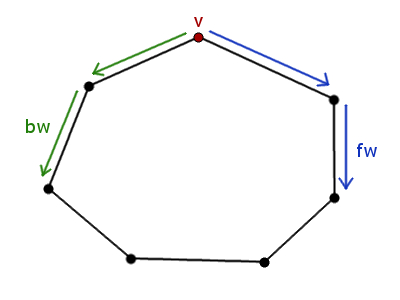
\includegraphics[scale = 0.6]{Resources/Images/diagram.jpg}
\end{center}
Algorytm wykorzystuje w tym celu dwa iteratory: w przód (forward, ozn. \textbf{fw}) oraz w tył (backward, ozn. \textbf{bw}). Jest to możliwe dzięki zastosowaniu list dwukierunkowych na wierzchołki i krawędzie w implementacji klasy Polygon (reprezentującej wielokąt).\\[\baselineskip]
Iterator \textbf{fw} próbuje dopasować wierzchołki końcowe krawędzi do początkowych (stosuje ograniczenie ``w przód''), natomiast iterator \textbf{bw} dopasowuje wierzchołki początkowe krawędzi do końcowych (stosuje ograniczenie ``w tył'').\\[\baselineskip]
Aplikowanie ograniczeń krawędzi zostaje przerwane, jeżeli iteratory się spotkają lub będą na incydentnych krawędziach. Po wykonaniu pełnej pętli następuje sprawdzenie, czy wszystkie ograniczenia są zachowane. Jeżeli nie, zapamiętane na początku położenie wierzchołków zostaje przywrócone. W programie objawia się to ``zablokowanym'' wielokątem, tzn. danego ruchu nie można wykonać, bo według algorytmu spowodowałby zepsucie ograniczeń.\\[\baselineskip]
\textbf{Pseudokod}
\begin{verbatim}
  1.  zapamiętaj położenie wierzchołków w wielokącie
  2.  fw = krawędź, której wierzchołek początkowy == v
  3.  bw = krawędź, której wierzchołek końcowy == v
  4.  while (true)
  5.      zastosuj ograniczenie krawędzi w iteratorze fw w przód
  6.      zastosuj ograniczenie krawędzi w iteratorze bw w tył
  7.      break, jeżeli krawędź w fw == krawędź w bw
  8.      fw = fw.Next lub pierwszy element listy krawędzi,
               jeżeli doszliśmy do końca
  9.      break, jeżeli krawędź w fw == krawędź w bw
  10.     bw = bw.Prev lub ostatni element listy krawędzi,
               jeżeli doszliśmy do początku
  11. sprawdź ograniczenia i przywróć położenie wierzchołków,
          jeżeli jakieś nie jest zachowane
\end{verbatim}

\end{document}